\documentclass[deutsch]{llncs}
\usepackage{multirow, cellspace}
\usepackage{microtype}
\usepackage{tabularx}
\usepackage{ltablex}
\usepackage{amssymb}
\usepackage{amsmath}
\usepackage[utf8]{inputenc} %Umlaute
\usepackage{amssymb}
\usepackage{upgreek}
\usepackage{graphicx}
\usepackage{amsmath}

\renewcommand{\arraystretch}{1.5}
\setlength{\jot}{10pt}

\begin{document}

\title{Intelligente Sehsysteme - Übungsblatt 1}


\author{Jan Konrad (2533619)}
\institute{}
\maketitle

\section*{Aufgabe 2}
Lösung für $k=G$ und $a=3$:\\
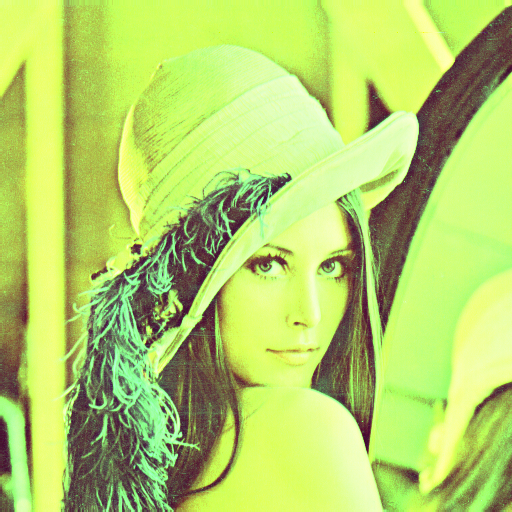
\includegraphics[width=\textwidth]{G3.png}

\section*{Aufgabe 3}
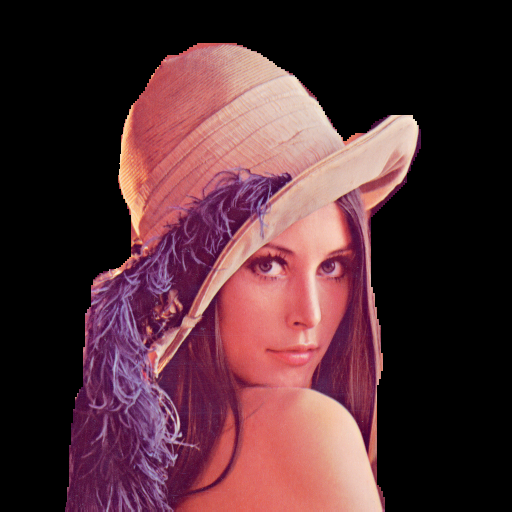
\includegraphics[width=\textwidth]{mask.png}

\section*{Aufgabe 4}
\begin{enumerate}
	\setlength\itemsep{1em}
	\item
	      \begin{tabular}{ |c| c c c c c c c c| }
		      \hline
		      $\mathbf{I}$      & 0 & 1 & 2 & 3 & 4 & 5 & 6 & 7 \\
		      \hline
		      $h(\mathbf{I_1})$ & 0 & 3 & 5 & 2 & 3 & 2 & 1 & 0 \\
		      \hline
		      $h(\mathbf{I_2})$ & 1 & 7 & 4 & 0 & 0 & 0 & 3 & 1 \\
		      \hline
	      \end{tabular}

	\item
	      \begin{tabular}{ |c| c c c c c c c c| }
		      \hline
		      $\mathbf{I}$      & 0      & 1      & 2      & 3     & 4      & 5     & 6      & 7      \\
		      \hline
		      $p(\mathbf{I_1})$ & 0      & 0.1875 & 0.3125 & 0.125 & 0.1875 & 0.125 & 0.0625 & 0      \\
		      \hline
		      $p(\mathbf{I_2})$ & 0.0625 & 0.4375 & 0.25   & 0     & 0      & 0     & 0.1875 & 0.0625 \\
		      \hline
	      \end{tabular}

	\item $m_{\mathbf{I_1}}=2.9375$
	      , $m_{\mathbf{I_2}}=2.5$
	      , $q_{\mathbf{I_1}}\approx 1.5194$
	      , $q_{\mathbf{I_2}}\approx 2.2361$

	\item Aus $m_{\mathbf{I_1}} \approx m_{\mathbf{I_2}}$ lässt sich ableiten,
	      dass im Mittel beide Bilder ungefähr gleich hell sind, wobei $m_{\mathbf{I_2}}$ etwas dunkler ist.
	      Aus $q_{\mathbf{I_2}} > q_{\mathbf{I_1}}$ folgt,
	      dass der Kontrast von $\mathbf{I_2}$ höher als der Kontrast von $\mathbf{I_1}$ ist.
	      Bei der Auswertung muss beachtet werden, dass das Bild $\mathbf{I_2}$ bimodal verteilt ist. D.h. es gibt zwei klar getrennte Bereiche.
	      Die örtliche Anordnung der Intensitätswerte kann aus den Werten nicht abgeleitet werden.

\end{enumerate}

\section*{Aufgabe 5}
\begin{enumerate}
	\setlength\itemsep{1em}
	\item
	      \begin{tabular}{ |c| c c c c c c c c| }
		      \hline
		      $\mathbf{I}$    & 0 & 1 & 2 & 3 & 4 & 5 & 6 & 7 \\
		      \hline
		      $h(\mathbf{I})$ & 0 & 0 & 2 & 2 & 2 & 2 & 0 & 0 \\
		      \hline
	      \end{tabular}

	\item
	      \begin{tabular}{ |c| c c c c c c c c| }
		      \hline
		      $\mathbf{I}$    & 0 & 1 & 2    & 3    & 4    & 5    & 6 & 7 \\
		      \hline
		      $p(\mathbf{I})$ & 0 & 0 & 0.25 & 0.25 & 0.25 & 0.25 & 0 & 0 \\
		      \hline
	      \end{tabular}

	\item  Bei der linearen Histogrammspreizung $T(\mathbf{I})$ wird das Histogramm zuerst nach links verschoben,
	      s.d. $\mathbf{I}_{minGiven} = \mathbf{I}_{min}$ gilt.
	      Anschließend wird das Historgram skaliert, s.d. $\mathbf{I}_{maxGiven} = \mathbf{I}_{max}$ gilt.\\
	      Für $\mathbf{I}_{min} = 0$ gilt für $T(\mathbf{I})$ demnach Folgendes:

	      \begin{equation*}
		      \begin{split}
			      c_1& = - \mathbf{I}_{minGiven} = -2 \\
			      c_2& = \frac {\mathbf{I}_{max}} {\mathbf{I}_{maxGiven}-\mathbf{I}_{minGiven}} = \frac {7}  {5 - 2} = \frac{7}{3} \\
			      T(\mathbf{I}) & = (\mathbf{I} + c_1) \cdot c_2 \\
			      &= (\mathbf{I} -2) \cdot \frac{7}{3}
		      \end{split}
	      \end{equation*}

	      Da es sich hier um ein diskretes Histogramm handelt, wird $T(\mathbf{I})$ gerundet.

	\item
	      \begin{math}
		      \mathbf{I}^\prime = T(\mathbf{I}) =
		      \begin{tabular}{ |c|c|c|c| }
			      \hline
			      0 & 2 & 2 & 7 \\
			      \hline
			      0 & 5 & 5 & 7 \\
			      \hline
		      \end{tabular}
	      \end{math}
\end{enumerate}

\section*{Aufgabe 6}
\begin{enumerate}
	\setlength\itemsep{1em}
	\item
	      \begin{math}
		      \mathbf{I}^\prime = T_{\gamma=0.5}(\mathbf{I}) =
		      \begin{tabular}{ |c|c|c|c| }
			      \hline
			      0 & 3 & 3 & 6 \\
			      \hline
			      0 & 4 & 4 & 6 \\
			      \hline
		      \end{tabular}
	      \end{math}

	\item
	      \begin{math}
		      \mathbf{I}^\prime = T_{\gamma=2}(\mathbf{I}) =
		      \begin{tabular}{ |c|c|c|c| }
			      \hline
			      0 & 0 & 0 & 3 \\
			      \hline
			      0 & 1 & 1 & 3 \\
			      \hline
		      \end{tabular}
	      \end{math}

	\item Für $\gamma > 1$ werden hohe Intensitätswerte gespreizt und niedrige Intensitätswerte gestaucht.
	      Das Gegenteil gilt für $\gamma < 1$.\\
	      Das Bild  $\mathbf{I}$ ist ein unterbelichtetes Bild (Mehrheit der Intensitätswerte ist niedrig),
	      daher ist eine Korrektur mit $\gamma = 0.5$ sinnvoller.
	      Bei dieser Korrektur wird mit $\{0, \ldots, 6  \}$ fast das gesamte Spektrum genutzt.
	      Bei einer Korrektur mit $\gamma = 2$ wird das genutze Spektrum dagegen sogar kleiner.
\end{enumerate}

\section*{Aufgabe 7}
\begin{enumerate}
	\setlength\itemsep{1em}
	\item
	      \begin{tabular}{ |c| c c c c c c c c| }
		      \hline
		      $\mathbf{I}$    & 0 & 1 & 2 & 3 & 4 & 5 & 6 & 7 \\
		      \hline
		      $h(\mathbf{I})$ & 1 & 2 & 1 & 0 & 0 & 0 & 2 & 2 \\
		      \hline
	      \end{tabular}

	\item
	      \begin{tabular}{ |c| c c c c c c c c| }
		      \hline
		      $\mathbf{I}$    & 0     & 1    & 2     & 3 & 4 & 5 & 6    & 7    \\
		      \hline
		      $p(\mathbf{I})$ & 0.125 & 0.25 & 0.125 & 0 & 0 & 0 & 0.25 & 0.25 \\
		      \hline
	      \end{tabular}

	\item
	      \begin{tabular}{ |c| c c c c c c c c| }
		      \hline
		      $\mathbf{I}$    & 0     & 1     & 2   & 3   & 4   & 5   & 6    & 7 \\
		      \hline
		      $s(\mathbf{I})$ & 0.125 & 0.375 & 0.5 & 0.5 & 0.5 & 0.5 & 0.75 & 1 \\
		      \hline
	      \end{tabular}

	\item
	      \begin{math}
		      \mathbf{I}^\prime = T_H(\mathbf{I}) =
		      \begin{tabular}{ |c|c|c|c| }
			      \hline
			      1 & 3 & 3 & 7 \\
			      \hline
			      4 & 6 & 6 & 7 \\
			      \hline
		      \end{tabular}
	      \end{math}
\end{enumerate}
\end{document}
